\chapter{}
Dos irmãos Filpi, apenas três cursaram faculdade: Tio Ângelo, o mais velho e Tio Zico, o mais novo, diplomados em Medicina e Tio Bepe, que se tornou farmacêutico.
Papai e Tio Totó chegaram apenas até a sétima série, quando foram bruscamente tirados da escola para ajudar na roça.
Apesar disso, viraram-se tão bem na vida quanto os irmãos formados.
Se Papai alcançou uma solidez financeira maior, foi porque Tio Totó explorou mais entusiasticamente sua verve política do que sua habilidade para os negócios.
Mas os irmãos homens, diplomados ou não, ganhavam o suficiente para uma vida confortável.
Mesmo Tio Bepe, um boa-vida contumaz, sustentava-se dando nome a uma ou duas farmácias tocadas por práticos, que ele avalizava com o seu diploma.
A preocupação maior dos irmãos homens eram as irmãs, criadas pela mãe no borralho e que eles sentiam ter o dever de resgatar do atraso, familiarizando-as com os hábitos da vida urbana e com as conquistas da modernidade.
Papai, principalmente, o tempo todo instado pela inconformidade da minha mãe com a sorte das cunhadas, levava-as passear constantemente.
Essa era a razão porque durante boa parte da sua vida, ele só teve esse tipo de carro conhecido como ``perua''.


Quase todos os domingos, buscávamos as tias para levá-las a conhecer as cidades das redondezas, para comer num restaurante, ou visitar uma atração turística qualquer.
Também fomos algumas vezes a Santos para que vissem o mar.
Nós, as crianças, aprovávamos entusiasmados tais iniciativas não só porque gostávamos muito delas e dos passeios, mas também porque dado o fato de as estradas asfaltadas serem raridade ainda, estas viagens demoravam tempo suficiente para justificar a enorme cesta de sanduíches, sucos, pastéis e bolos que as tias preparavam ``para a gente encostar o estômago'' no trajeto.

\begin{figure}[H]
\centering
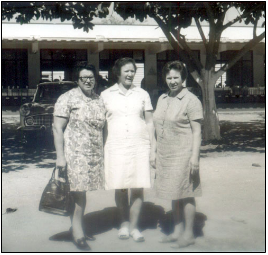
\includegraphics[width = 0.6\linewidth]{9/tias-1.png}
\caption{Tia Imaculada, Tia Glória e Tia Antonieta, num passeio de domingo.}
\end{figure}

Um belo dia, Tio Ângelo quis que elas fossem visitá-lo no Rio.
Ele tinha construído uma enorme casa na praia de Sepetiba como contrapartida à remoção do centro de umbanda da sua mulher para aquele subúrbio e aproveitou para estender o convite a toda a família.
Passaríamos o Natal lá, naquele tempo uma idílica colônia de pescadores, ainda.
Devíamos ir todos, desde o recém-nascido Joãozinho, meu irmão, até Tio Zé e Tia Yolanda, sempre arredios.


O comboio partiu de Araraquara com uma semana de antecedência.
À frente ia a nossa Kombi, porque Papai era um bom conhecedor das estradas, levando nossa família, Tia Imaculada, Tia Glória, Tia Neta e uma parte substancial da merenda, para nossa alegria.
No meio, seguia o caminhão do Tio Totó carregando sacos de frutas, de arroz, de feijão, de milho-verde, engradados de frangos, porcos e cabritos vivos, tudo envolto num inacreditável amarrado de lona que não podia ser muito fechado para não sufocar os animais, mas, ao mesmo tempo, devia ocultar suficientemente a carga para não causar embaraços com a polícia rodoviária, que certamente não acreditaria quando dissessem que tudo aquilo se destinava a mitigar os gastos dos anfitriões com a alimentação daquele bando de glutões.
Desse arranjo resultou que logo no primeiro solavanco da estrada de terra (o asfalto só começava cerca de uma centena de quilômetros antes de São Paulo), parte da lona se desprendeu e para garantir que ela não voasse de vez, assentaram sobre a carga os cento e trinta quilos do Tio Bepe, o que teve a vantagem adicional de desapertar a cabine onde se espremiam Tio Totó e Tia Albina, outra gordinha.
Como Tio Bepe estava ficando careca, amarraram-lhe sobre o cocuruto um lenço à moda dos paisanos da velha Itália, com nós nas quatro pontas para um melhor ajuste anatômico.
E lá seguiu a geringonça, lona enfunada qual uma caravela sobre rodas, ornada no topo pela imensa figura na qual se misturavam em estranha combinação a elegância do terno, de que Tio Bepe jamais abria mão, mais o lenço branco arrematando aquele carão arroxeado pelo maçarico de um sol de dezembro.

Fechando o cortejo, arfando, seguia a ``ximbica'' do Tio Zé, um Fordinho 29 na versão utilitária que um dia, como se depreendia das pequenas manchas visíveis aqui e acolá entre as grandes extensões de tinta de fundo, fora de um belo azul-celeste.
Esta viatura caracterizava-se por ser um primor da criatividade cabocla que o Tio Zé tão bem representava.
A ignição, eu me lembro, era dada por meio de uma chave elétrica dessas montadas numa base de cerâmica, como as que ligavam as máquinas do meu pai, na fábrica.
Era uma adaptação de que Tio Zé se orgulhava por superar em muito, de acordo com ele, a rasteira eficiência das partidas originais de fábrica.
O assoalho, que de há muito apodrecera de ferrugem, fora habilidosamente substituído por tábuas de madeira por cujos vãos se acompanhava a passagem da estrada sob as rodas, vantagem que compensava de sobra os banhos que a tia levava quando atravessavam as poças de água ou lama.
Os faróis também mereceram um importante melhoramento resultante de horas de pesquisa daquele gênio matuto.
Por via das dúvidas, decidiu-se não viajar à noite, porque embora o Tio gabasse a qualidade indiscutível daqueles holofotes adaptados, a verdade é que eles não iluminavam mais do que velas de sebo.
Havia muitas outras intervenções que a minha pouca familiaridade com a mecânica de carros me impedia de alcançar na época, muito embora Tio Zé não se importasse de explicá-las didaticamente a quem se interessasse e até demonstrasse um enorme prazer em fazê-lo.
Mas o mais preocupante de tudo era ele mesmo, o motorista.
Tio Zé tinha inexplicável atração por barrancos.
Tinha o vezo de por nada, assim que divisava lá longe a aproximação de um carro na direção contrária, arremeter para fora do caminho, o que acabou por conferir à pobre “ximbica” aquele aspecto de camuflada.
As consequências só não eram mais catastróficas porque ela rodava muito devagar em virtude de outra criação do Tio Zé destinada a economizar combustível.
Ela quase não gastava, mas também não andava.
Assim, a cada trecho, parávamos no acostamento e rezávamos contritamente por cerca de quarenta minutos até que percebíamos no horizonte aquele pontinho negro movendo-se como cavalo passarinheiro para lá e para cá na estrada.
Aliviados íamos adiante, seguros de que eles ainda nos seguiam.
A todas essas, Tia Yolanda, sentada ao lado do marido, mantinha a dignidade de uma dama inglesa a bordo do seu Rolls-Royce.

É bem verdade que o caminhão do Tio Totó também não era grande coisa.
Meu tio era famoso pela displicência com seus veículos.
Um farol apenas lhe bastava, freio de mão era supérfluo porque ele nunca se lembrava de acioná-lo quando parava num lugar qualquer da sua Boa Esperança.
Estacionar também estava fora de questão.
Quando lhe dava na telha, apeava no meio da rua, como quem desmontasse de um cavalo e nem se dava ao trabalho de fechar a porta, ou retirar as chaves.
O que facilitava para os munícipes a tarefa de deter o carro quando começava a rolar rua abaixo.
Seu genro conta que ele encheu de leitõezinhos vivos para levar para a fazenda, um sedã retirado um dia antes da concessionária, novinho em folha.
Na rodovia que o levava da cidade à fazenda, mal se pilhava numa reta, adormecia.
Acordava-o um cutucão da Tia Albina ou, se ele estivesse sozinho, o solavanco do carro saindo da pista para o acostamento.
Repunha o carro no prumo e voltava a dormir.
Quando íamos com ele para a fazenda, as tias nos instruíam a fazer todo o barulho possível para evitar os cochilos.
Contudo, milagrosamente, Tio Totó só sofreu dois acidentes de monta em toda sua vida: um, quando dormindo, como sempre, errou a ponte e focinhou no rio Jacaré e outro, o acidente que o matou, já nonagenário, quando, ao que tudo indica, enfartou dirigindo.

 
Em Aparecida do Norte, meio da viagem, mais ou menos, fizemos um pouso.
As tias queriam conhecer a basílica da santa milagrosa.
A visita nos tomou a manhã do dia seguinte, de modo que resolvemos almoçar por ali.
O pedido no restaurante foi exagerado, mesmo pelos padrões dos Filpi, e assim sobraram três frangos assados que Tio Bepe mandou embrulhar e que, tão logo reassumiu seu posto sobre a carroceria do caminhão, pôs-se a saborear calmamente, a pretexto de que o tinham apressado demais durante a refeição.
E, por falar em exagero, Pepone parece ter achado excessiva também a gorjeta que meu pai e Tio Totó deixaram sobre a mesa, de modo que, deixando-se ficar por último à saída, tratou de corrigir o despropósito, metendo no bolso dois terços das cédulas.
Quando retornamos à estrada, suponho que intrigado com o aspecto esquisitíssimo da carga mal ajambrada, encimada por aquela paquidérmica criatura de terno atracada aos seus frangos, um guarda fez sinais frenéticos para que o caminhão parasse.
Tio Totó, porém, avançou impavidamente, lona a todo o pano, largando para trás o sujeito espumando de ódio impotente.

Ao fim da viagem, já ao anoitecer, fomos festivamente recebidos pelos tios à porta da casa que mais parecia um pequeno hotel.
Eram catorze quartos cheios de beliches e fartamente abastecidos com ventiladores e bombas de inseticida.
Três horas depois, banhados, jantados e finalmente adormecidos, descobrimos o porquê das medidas preventivas: acordamos sob o ataque do mais formidável exército de pernilongos que eu jamais experimentei em toda minha vida, em qualquer canto desse país.
 Isso em meio a um lago de suor que nos ensopava os pijamas e os lençóis.
Um suplício completo.
Onde estavam os ventiladores, perguntávamos de quarto em quarto, nos debatendo entre as nuvens daquelas minúsculas e sanguinárias feras e o cheiro intenso do veneno espalhado pelo ar.
Tinham misteriosamente desaparecido.
Ninguém conseguia mais ficar na cama.
Apenas um quarto, entre todos, permaneceu fechado: o do Tio Bepe.
Invejosos da insensibilidade daquele bruto que conseguia dormir naquele inferno, passamos o resto da noite a caminhar e a nos abanar até que, pelo amanhecer, decidimos ir deitar na areia da praia.
Na volta, encontramos Tia Neta furibunda: fora arrumar a cama do gordo e, acreditem, ao redor da cama dele ainda funcionavam a plena carga todos os ventiladores desaparecidos! 

\begin{figure}[H]
\centering
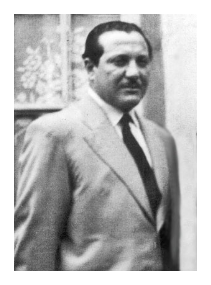
\includegraphics[width = 0.6\linewidth]{9/pepone.png}
\caption{O garboso Pepone, quando jovem.}
\end{figure}

E essa seria só mais uma das muitas gracinhas perpetradas por aquele folgado.
Em dois dias, como acontece desde sempre nas pequenas cidades praieiras do nosso país, o abastecimento de água entrou em colapso.
Tio Ângelo imediatamente contratou um caminhão pipa para encher os reservatórios da casa todas as manhãs.
Para beber, ele trazia engradados de água mineral, à tardinha, quando vinha do Rio.
Contudo, o caminhão pipa, dado o excesso de demanda, não era muito pontual e um dia, voltando da praia, mortos de sede naquele calor, descobrimos que não havia em toda a casa uma única gota de água.
Exceto num lugar, conforme voltou anunciando Tia Neta, que se afastara para investigar o fenômeno, já intuindo a causa: lá fora, num cercadinho improvisado em banheiro, um Tio Bepe feliz da vida acabava de enxaguar seu agora refrescado corpanzil com a última garrafa de água mineral dos dois engradados inteiros que usara para tomar seu banho matinal.
Língua de fora, tivemos que peregrinar de boteco em boteco da vilazinha atrás de água para beber, até que Tio Ângelo chegasse à noite com um novo suprimento.

Nunca entendi porque, mas Tio Bepe, entre os irmãos, gozava de uma inimputabilidade de índio.
Tanto que por muito tempo pensei que ele fosse o mais novo.
Não era.
Aliás, estava entre os mais velhos.
Só não lhe achavam graça Tia Neta, a rebelde, e Tio Zico, esse sim, o caçula dos homens.
Tanto que, num outro dia, deparamo-nos com este último aos berros, apoplético, ameaçando beber o sangue daquele gordo parasita.
Pois ele, Zico, tinha trazido da famosa confeitaria Colombo, a peso de ouro, alguns quilos de uma azeitona espanhola recheada, com a intenção de servi-los aos irmãos como aperitivo para o almoço.
Para tanto, deixara a praia mais cedo, a tempo de certificar-se de que tudo estava preparado e as bebidas devidamente geladas.
Qual não foi sua indignação quando divisou Tio Bepe no terraço, refestelado na espreguiçadeira, ao lado do pote das preciosas azeitonas e cercado de garrafas vazias de cerveja.
Aquele Pantagruel tinha devorado quase todas as azeitonas sozinho e ainda reforçara o ato criminoso com uma verdadeira devastação no estoque de bebida gelada.
Daquela vez, Pepone escapou por pouco de ser lançado por cima da balaustrada.
Livrou-o a chegada dos irmãos que a custo seguraram o mais novo, tomado de ódio assassino.

Uma noite, um pouco antes do fim da temporada, Tia Mariazinha, a anfitriã, brindou-nos com uma sessão no seu recém-inaugurado centro de umbanda.
Exibição magnífica de ritmos e cores.
Lá pelas tantas, as entidades já incorporadas nos seus respectivos cavalos aproximaram-se dos visitantes para dar-lhes o passe de preceito.
Os irmãos Filpi foram enfileirados em ala e o que se seguiu foi para minha mãe a mais inesquecível recordação dessa viagem e a comprovação inequívoca e para sempre lembrada de tudo quanto ela dizia a respeito do gênio selvagem da família do marido: apenas iniciado o ritual, como pedras de um dominó, os caboclos foram caindo para trás duros e tesos, como que fulminados por raio.
Mamãe voou para a porta e foi estourar de riso lá fora, protegida pela escuridão.

\begin{figure}[H]
\centering
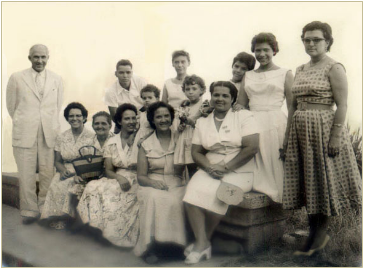
\includegraphics[width = 0.6\linewidth]{9/viagem-a-sepetiba.png}
\caption{Uma lembrança da viagem a Sepetiba: as tias, primos e nossos anfitriões, Tio Ângelo, de pé à esquerda e Tia Mariazinha, sentada à direita, de colar e costume branco.
Na extrema direita, Tia Ilka, a mulher do Tio Zico.}
\end{figure}


Passado o Ano Novo, voltamos para Araraquara e certamente ficou por muito tempo na memória dos caiçaras de Sepetiba a lembrança daqueles alienígenas que lhes consumiram toda a produção de peixe e camarão daqueles dias, pagando nababescamente por isso, bem como a estranha aparição dos tios fazendeiros, madrugadinha ainda, para acompanhar a saída dos barcos, entrando mar adentro de chapelão boiadeiro, camisa de mangas longas abotoada até o pescoço, calção, meias e botinas de elástico.
Todos os dias, enquanto lá estivemos.

As tias conheceram uma das suas poucas férias de Natal.
Porque enquanto puderam reunir os irmãos, era na casa delas que essa festa acontecia.
Da véspera do dia vinte e cinco de dezembro até o dia dois de janeiro, elas se revezavam num absurdo mutirão destinado a manter cheio o prato de no mínimo quatro ou cinco dezenas de pessoas que mal se levantavam da cadeira entre uma refeição e outra.